\documentclass[preprint,12pt]{elsarticle}
\makeatletter
\def\ps@pprintTitle{%
   \let\@oddhead\@empty
   \let\@evenhead\@empty
   \def\@oddfoot{August\enspace2018}%
   \def\@evenfoot{August\enspace2018}%
}

\makeatother

\usepackage{amsmath, amsthm, amssymb, amsfonts, tikz, caption, subcaption, python, program}
\usepackage{pgfplots}
\usepackage{algorithm}
\usepackage[noend]{algpseudocode}
\usetikzlibrary{matrix,chains,positioning,decorations,arrows}
\usetikzlibrary{matrix,chains,positioning,decorations.pathreplacing,arrows,calc}

\def\layersep{2.5cm}

\tikzset{
block/.style={
  draw,
  rectangle, 
  text width=3em, 
  text centered, 
  minimum height=8mm,     
  node distance=2.3em
  }, 
line/.style={draw}
}

%% Use the option review to obtain double line spacing
%% \documentclass[preprint,review,12pt]{elsarticle}

%% Use the options 1p,twocolumn; 3p; 3p,twocolumn; 5p; or 5p,twocolumn
%% for a journal layout:
%% \documentclass[final,1p,times]{elsarticle}
%% \documentclass[final,1p,times,twocolumn]{elsarticle}
%% \documentclass[final,3p,times]{elsarticle}
%% \documentclass[final,3p,times,twocolumn]{elsarticle}
%% \documentclass[final,5p,times]{elsarticle}
%% \documentclass[final,5p,times,twocolumn]{elsarticle}

%% The graphicx package provides the includegraphics command.
\usepackage{graphicx}
%% The amssymb package provides various useful mathematical symbols
\usepackage{amssymb}
%% The amsthm package provides extended theorem environments
%% \usepackage{amsthm}

%% The lineno packages adds line numbers. Start line numbering with
%% \begin{linenumbers}, end it with \end{linenumbers}. Or switch it on
%% for the whole article with \linenumbers after \end{frontmatter}.
%%\usepackage{lineno}

%% natbib.sty is loaded by default. However, natbib options can be
%% provided with \biboptions{...} command. Following options are
%% valid:

%%   round  -  round parentheses are used (default)
%%   square -  square brackets are used   [option]
%%   curly  -  curly braces are used      {option}
%%   angle  -  angle brackets are used    <option>
%%   semicolon  -  multiple citations separated by semi-colon
%%   colon  - same as semicolon, an earlier confusion
%%   comma  -  separated by comma
%%   numbers-  selects numerical citations
%%   super  -  numerical citations as superscripts
%%   sort   -  sorts multiple citations according to order in ref. list
%%   sort&compress   -  like sort, but also compresses numerical citations
%%   compress - compresses without sorting
%%
%% \biboptions{comma,round}

% \biboptions{}

\journal{Journal Name}

\begin{document}

\begin{frontmatter}

%% Title, authors and addresses

\title{ConstellationCV: Obtaining 3D Information from 2D Images Efficiently using Feature Extraction and Laser Dot Projection}

%% use the tnoteref command within \title for footnotes;
%% use the tnotetext command for the associated footnote;
%% use the fnref command within \author or \address for footnotes;
%% use the fntext command for the associated footnote;
%% use the corref command within \author for corresponding author footnotes;
%% use the cortext command for the associated footnote;
%% use the ead command for the email address,
%% and the form \ead[url] for the home page:
%%
%% \title{Title\tnoteref{label1}}
%% \tnotetext[label1]{}
%% \author{Name\corref{cor1}\fnref{label2}}
%% \ead{email address}
%% \ead[url]{home page}
%% \fntext[label2]{}
%% \cortext[cor1]{}
%% \address{Address\fnref{label3}}
%% \fntext[label3]{}


%% use optional labels to link authors explicitly to addresses:
%% \author[label1,label2]{<author name>}
%% \address[label1]{<address>}
%% \address[label2]{<address>}

\author{\text{Pratham Gandhi (pratham\_gandhi@horacemann.org)}}
\author{\text{Samuel Schuur (samuel\_schuur@horacemann.org)}}

\address{Bronx, New York}

\begin{abstract}
%% Text of abstract
In this paper, the development and application of a system to computationally inexpensively determine a three dimensional model of a space from only a single image is presented, using applied machine learning and simple hardware components. Using feature classification of the relevant objects in the original scene, in collection with a physical grid of laser dots refracted across the scene, the system is able to quickly judge the nature of the object, its position in relation to other objects around it, and distance of those objects from the camera, traits which are commonly compromised on comparable approaches. The system is \begin{it}x\end{it} times more efficient on average than current industry leading approaches, and has potential applications in various fields requiring rapidly updating spatial awareness and environment generation, including autonomous vehicles, defense, and architecture.
\end{abstract}

%%\begin{keyword}
%% keywords here, in the form: keyword \sep keyword

%% MSC codes here, in the form: \MSC code \sep code
%% or \MSC[2008] code \sep code (2000 is the default)

%%\end{keyword}


\end{frontmatter}
\pagebreak

%%
%% Start line numbering here if you want
%%

%% main text
\section{Introduction}
\label{S:1}
The current most popular approach to creating a three dimensional informational estimate from a two dimensional image is triangulation, or binocular, stereo vision approach. This approach take several images of the same scene from different locations and angles in order to generate a spatial awareness. Computer stereo vision, however, is difficult to implement in practical applications in our increasingly evolving digital world, due to the limiting factor that they require multiple images, the acquisition of which is sometimes impractical. Additionally, they can sometimes be quite slow, in that they need to first identify common features in the different photos, find out the positional relation of those features, and then only begin to start seeing the greater picture of the full space. The purpose of Constellation was to solve both of these problems and create a flexible system which can adapt and continue to be functional in many environments.

We chose to approach this problem first through the somewhat traditional technique of using artificial neural networks, mathematical functions modeled after nature which specialize in taking in large amounts of input to produce outputs, to identify features in a two dimensional image. Neural networks are are perfect for navigating the fuzzy problems of feature extraction from images. Where our system differs is in its use of a grid of refracted laser points into the scene to judge the distances and orientations of various objects in relation to the camera. This allows superior environment generation in a shorter amount of time, due to the omission of the multiple-image stereo aspect. This approach and its implemented system was named Constellation for the star-like appearance of the laser dot grid it relies on.

\section{Background}
\label{S:2}
\subsection{Binocular Computer Stereo Vision}
In order to perceive depth the human eye uses many visual cues, both monocular and binocular. Of these visual cues, stereopsis, the perception of depth resulting from the brain comparing the differences in images produced by both eyes, is in many ways one of the easiest depth perceptions methods to mimic through software, as it is the least reliant on external sources of stimuli and human experience. This is what Stereo Computer Vision attempts to do; building depth maps by comparing scenes from multiple vantage points. More specifically Binocular Computer Stereo Vision does this by comparing the images from two cameras and by extracting and comparing common features from both images it builds a depth map of the scene in question.

\subsubsection{Removing Distortion from Images}
Modern cameras introduce two major kinds of distortion to their images: barrel distortion and tangential distortion. Barrel distortion, a form of radial distortion, is introduced due to the curvature of lenses and, as such, is more prominent in wider angle lenses. Barrel distortion causes objects toward the edges of the frame to appear smaller than objects in the middle of the frame, therefore creating a situation where distances in relation to the size of an object are nonlinear. Tangential distortion on the other hand is introduced due to the lens of a given camera not being properly aligned with the imaging sensor, causing some areas of the image to look larger than others, once again causing the relationship between size and distance to be nonlinear. However, since binocular computer vision requires that the distance-size relationship must remain consistent throughout an image to be able to accurately compare images from different positions, these distortions must be corrected for, in order to effectively allow our camera to mimic the perfect pinhole camera.

In order to correct for radial and tangential distortion, many models and formulas have been proposed and developed, but for the purpose of this paper we will be using formulas derived from the Brown-Conrady model. The formulas for correcting radial distortion read as follows, where r is the distance from the distortion center to a distorted point:

$$x_{corrected} = x(1+k_1 r^2 + k_2 r^4 + k_3 r^6)$$
$$y_{corrected} = x(1+k_1 r^2 + k_2 r^4 + k_3 r^6)$$

So a pixel (x, y) in the distorted image will be remapped to ($x_{corrected}$, $y_{corrected}$). The same is true in the following formulas for correcting tangential distortion:

$$x_{corrected} = x + (2p_1 x y + p_2(r^2 + 1x^2))$$
$$y_{corrected} = y + (p_1(r^2 + 2y^2) + 2p_2 x y)$$

In above formulas are five distortion parameters that must be seperately experimentally determined in order to correct the image: $k_1, k_2, p_1, p_2,\text{and } k_3$. In addition to these, a given camera's "camera matrix" must be determined, which is a set of intrinsic camera parameters such as focal length and optical centers. This information is determined experimentally, on a camera to camera basis, by taking multiple images of a grid of objects of known size, shape, and relation to each other and tuning these parameters until the corrected grid matches the actual grid.
\subsubsection{Finding the epiline of an Image}
\subsubsection{Feature detecting and matching}
\subsubsection{Creating a depth map}
\subsection{Structure-From-Motion Pipelines}
\subsection{Structure-From-Motion Pipelines}
\subsection{Structure-From-Motion Pipelines}
\input{Diagrams/SFM.tex}
Structure-from-motion (SFM) pipelines operate on a simple premise; finding common anchor points among several images of the same subject, and using triangulation to estimate where those points lie in relation to the camera.
\subsubsection{Shortcomings}
One of the major issues in using SFM pipelines in practical applications where rapidly updating three dimensional estimations are required is that the models produced by SFM pipelines are lacking a scale factor, that is, there is no sense accurate of scale or distance in the model. This is one of the issues Constellation aims to address.
Structure-from-motion (SFM) pipelines operate on a simple premise; finding common anchor points among several images of the same subject, and using triangulation to estimate where those points lie in relation to the camera.
\subsubsection{Shortcomings}
One of the major issues in using SFM pipelines in practical applications where rapidly updating three dimensional estimations are required is that the models produced by SFM pipelines are lacking a scale factor, that is, there is no sense accurate of scale or distance in the model. This is one of the issues Constellation aims to address.
Structure-from-motion (SFM) pipelines operate on a simple premise; finding common anchor points among several images of the same subject, and using triangulation to estimate where those points lie in relation to the camera.
\subsubsection{Shortcomings}
One of the major issues in using SFM pipelines in practical applications where rapidly updating three dimensional estimations are required is that the models produced by SFM pipelines are lacking a scale factor, that is, there is no sense accurate of scale or distance in the model. This is one of the issues Constellation aims to address.
\subsection{Neural Networks}
A human brain is composed of billions of neurons, connected and excitable cells which allow humans to be intelligent. Each neuron's dendrites receive signals from other neurons. If the these electrical signals exceed a threshold, the neuron fires, thereby propagating a voltage out of its synapses and on to other neurons. Together, these neurons form an extensive network, where an immense set of sensory input i processed alongside expected outputs. The purpose of artificial neural networks is to simulate this same network of interconnected neurons using mathematical properties to emulate electrical signals and approximate complex functions
\subsubsection{Artificial Neurons}
\begin{figure}[h]
\centering
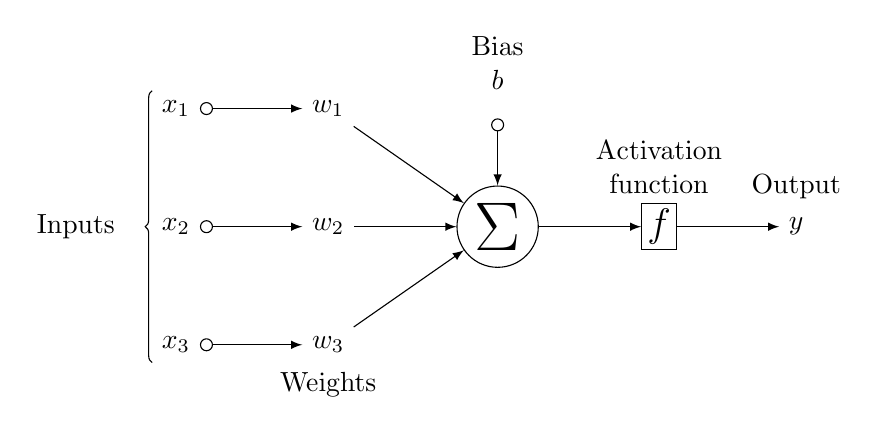
\begin{tikzpicture}[
init/.style={
  draw,
  circle,
  inner sep=2pt,
  font=\Huge,
  join = by -latex
},
squa/.style={
  draw,
  inner sep=2pt,
  font=\Large,
  join = by -latex
},
start chain=2,node distance=13mm
]
\node[on chain=2] 
  (x2) {$x_2$};
\node[on chain=2,join=by o-latex] 
  {$w_2$};
\node[on chain=2,init] (sigma) 
  {$\displaystyle\Sigma$};
\node[on chain=2,squa,label=above:{\parbox{2cm}{\centering Activation \\ function}}]   
  {$f$};
\node[on chain=2,label=above:Output,join=by -latex] 
  {$y$};
\begin{scope}[start chain=1]
\node[on chain=1] at (0,1.5cm) 
  (x1) {$x_1$};
\node[on chain=1,join=by o-latex] 
  (w1) {$w_1$};
\end{scope}
\begin{scope}[start chain=3]
\node[on chain=3] at (0,-1.5cm) 
  (x3) {$x_3$};
\node[on chain=3,label=below:Weights,join=by o-latex] 
  (w3) {$w_3$};
\end{scope}
\node[label=above:\parbox{2cm}{\centering Bias \\ $b$}] at (sigma|-w1) (b) {};

\draw[-latex] (w1) -- (sigma);
\draw[-latex] (w3) -- (sigma);
\draw[o-latex] (b) -- (sigma);

\draw[decorate,decoration={brace,mirror}] (x1.north west) -- node[left=10pt] {Inputs} (x3.south west);
\end{tikzpicture}
\caption{Artificial Neuron Diagram}
\end{figure}
An artificial neuron is an approximate mathematical model of a biological neuron, and is intended to fulfill similar purposes. Each artificial neuron has multiple inputs from other neurons. Along with the inputs, each neuron has a weight for each input, a bias term, and activation function, and only one output. The output of one neuron travels to other neurons and becomes of their inputs. The output of a neuron is expressed mathematically for $n$ inputs $x$ and weights $w$, a bias term $b$, and activation function $f(x)$ as follows:


$$activation = \sum\limits_{i=0}^n x_i w_i+b$$
$$output = f(activation)$$

Mentioned above, weights are positive or negative numbers which scale the effect or relevance of their accompanying inputs on a neuron's single output. Besides the weights, another important component of a neuron is the activation function, whose primary is to transform the output of a neuron. Common activation functions include a sigmoid curve, a hyperbolic tangent, a binary step function, and a rectifier function.The sigmoid activation and hyperbolic tangent activation functions are often used for general purpose neural networks due to their gradient nature, fixed range, and the fact that they are easily differentiated. Finally, the bias term is a number added to the summation of weighted inputs, which allows us to make transformations on the domain of the activation function.
\begin{figure}[h]
\centering
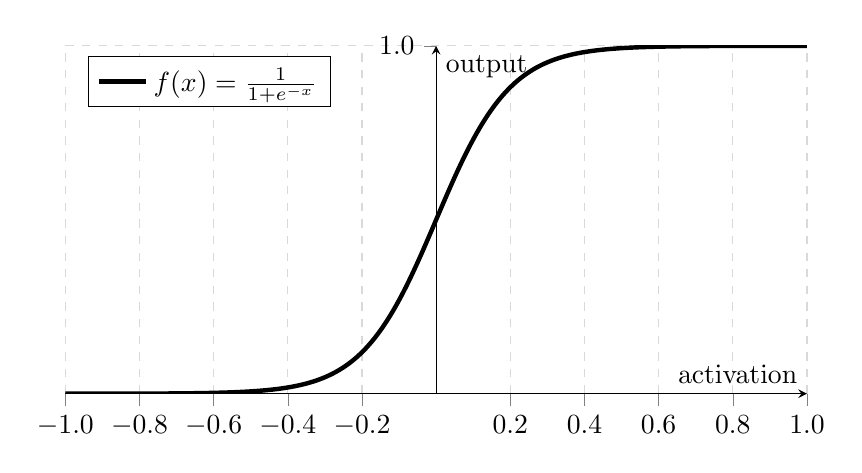
\begin{tikzpicture}
    \begin{axis}[
    	legend pos=north west,
        axis x line=middle,
        axis y line=middle,
        ytick={0,1},
        x tick label style={/pgf/number format/fixed,
                            /pgf/number format/fixed zerofill,
                            /pgf/number format/precision=1},
        y tick label style={/pgf/number format/fixed,
                            /pgf/number format/fixed zerofill,
                            /pgf/number format/precision=1},
        grid = major,
        width=11cm,
        height=6cm,
        grid style={dashed, gray!30},
        xmin=-1,     % start the diagram at this x-coordinate
        xmax= 1,    % end   the diagram at this x-coordinate
        ymin= 0,     % start the diagram at this y-coordinate
        ymax= 1,   % end   the diagram at this y-coordinate
        %axis background/.style={fill=white},
        xlabel=activation,
        ylabel=output,
        tick align=outside,
        enlargelimits=false]
      % plot the stirling-formulae
      \addplot[domain=-1:1, black, ultra thick,samples=500] {1/(1+e^(-10*x))};
      \addlegendentry{$f(x)=\frac{1}{1+e^{-x}}$}
    \end{axis}
\end{tikzpicture}
\caption{Sigmoid Function Graph}
\end{figure}
\subsubsection{Feed-forward Neural Network}
Constellation utilizes a feed-forward neural network, a collection of neurons organized into layers, as classifying mechanism for detection various features in a image. In a feed-forward neural network, the output of each neuron is the input of each neuron in the next layer. In this manner, the original inputs of the network are "fed forward" to new neurons in new layers, passing through a number of hidden layers in the middle, and finishing at the output layer.The outputs of the neurons in the final layer (output layer) are the outputs of the whole network and are used to judge the conclusion the network made.
\subsubsection{Backpropagation}
%\begin{figure}[h]
\centering
\begin{tikzpicture}[
    plain/.style={
      draw=none,
      fill=none,
      },
    net/.style={
      matrix of nodes,
     nodes={
       draw,
        circle,
    inner sep=10pt
    },
  nodes in empty cells,
  column sep=2cm,
  row sep=-9pt
  }, 
 >=latex
 ]
\matrix[net] (mat)
{ 
|[plain]| \parbox{1cm}{\centering Input\\layer} & |[plain]| \parbox{1cm}{\centering     Hidden\\layer} & |[plain]| \parbox{1cm}{\centering Output\\layer} \\
& |[plain]| \\
|[plain]| & \\
& |[plain]| \\
|[plain]| & |[plain]| \\
& & \\
|[plain]| & |[plain]| \\
& |[plain]| \\
|[plain]| & \\
& |[plain]| \\
};
\foreach \ai [count=\mi ]in {2,4,...,10}
  \draw[<-] (mat-\ai-1) -- node[above] {Input \mi} +(-2cm,0);
\foreach \ai in {2,4,...,10}
{\foreach \aii in {3,6,9}
  \draw[->] (mat-\ai-1) -- (mat-\aii-2);
}
\foreach \ai in {3,6,9}
  \draw[->] (mat-\ai-2) -- (mat-6-3);
%\draw[->] (mat-6-3) -- node[above] {Ouput} +(2cm,0);
\path [line] node{error} -- (mat-1-1);
\draw[->] (mat-6-3) -- ++(0pt,3cm) -| node[pos=0.15,above] {Error back propagation} ( $ (mat-2-1)!0.5!(mat-2-2) $ );
\end{tikzpicture}
\caption{A Feed-Forward Neural Network}
\end{figure} 

Supervised learning is the process of adjusting the weights of each neuron in a neural network in an effort to reach target outputs from a specific set of inputs, effectively "fine tuning" the neural network to make it as correct as possible. One of the most common methods of adjusting a neural network's weights is called backpropagation, first developed in Werbos in 1974.
\begin{figure}[h]
\centering
\tikzset{every picture/.style={line width=0.75pt}} %set default line width to 0.75pt        

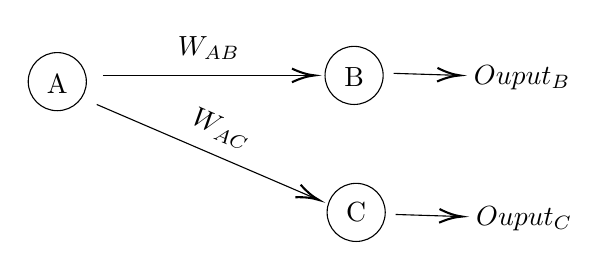
\begin{tikzpicture}[x=0.75pt,y=0.75pt,yscale=-1,xscale=1]
%uncomment if require: \path (0,300); %set diagram left start at 0, and has height of 300

\draw    (111, 74) circle [x radius= 14, y radius= 14]  ;
\draw    (130,85) -- (235.16,130.21) ;
\draw [shift={(237,131)}, rotate = 203.26] [color={rgb, 255:red, 0; green, 0; blue, 0 }  ][line width=0.75]    (10.93,-3.29) .. controls (6.95,-1.4) and (3.31,-0.3) .. (0,0) .. controls (3.31,0.3) and (6.95,1.4) .. (10.93,3.29)   ;

\draw    (255, 137) circle [x radius= 14, y radius= 14]  ;
\draw    (133,71) -- (233,71) ;
\draw [shift={(235,71)}, rotate = 180] [color={rgb, 255:red, 0; green, 0; blue, 0 }  ][line width=0.75]    (10.93,-3.29) .. controls (6.95,-1.4) and (3.31,-0.3) .. (0,0) .. controls (3.31,0.3) and (6.95,1.4) .. (10.93,3.29)   ;

\draw    (254, 71) circle [x radius= 14, y radius= 14]  ;
\draw    (273,70) -- (303,70.94) ;
\draw [shift={(305,71)}, rotate = 181.79] [color={rgb, 255:red, 0; green, 0; blue, 0 }  ][line width=0.75]    (10.93,-3.29) .. controls (6.95,-1.4) and (3.31,-0.3) .. (0,0) .. controls (3.31,0.3) and (6.95,1.4) .. (10.93,3.29)   ;

\draw    (274,138) -- (304,138.94) ;
\draw [shift={(306,139)}, rotate = 181.79] [color={rgb, 255:red, 0; green, 0; blue, 0 }  ][line width=0.75]    (10.93,-3.29) .. controls (6.95,-1.4) and (3.31,-0.3) .. (0,0) .. controls (3.31,0.3) and (6.95,1.4) .. (10.93,3.29)   ;


\draw (111,75) node  [align=left] {A};
\draw (255,137) node  [align=left] {C};
\draw (254,72) node  [align=left] {B};
\draw (184,58) node   {$W_{AB}$};
\draw (190,97) node [rotate=-23.81]  {$W_{AC}$};
\draw (335,72) node   {$Ouput_{B}$};
\draw (336,140) node   {$Ouput_{C}$};


\end{tikzpicture}
\caption{Single Branch of a Backpropagation Neural Network}
\end{figure}
In order to train neural networks through backpropagation (BP), we use examples. Each set of example inputs, known as training sets, are connected to a target output, which the system is aware of, and together the two parts form a training pair. The first step of training a BP network is to pass the training set through the neural network with randomly generated weights. The error, represented as $\delta$, for an output neuron is the difference between the actual output and the target output for that training set. Consider the abbreviated neural network illustrated in Figure 4. Assume this network has only an input layer consisting of an unspecified number of input neurons with unspecified outputs, a hidden layer containing only Neuron $A$, and an output layer consisting of Neurons $B$ and $C$. Obviously, $W_{AB}$ and $W_{AC}$ are the weights of the edges connecting the neurons. We complete the backpropagation action by modifying weight $W_{AB}$, replacing it with $W^+_{AB}$, as follows:
$$\delta_B=Target_B-Output_B$$
$$W^+_{AB}=W_{AB}+(\delta_B\times Output_A)$$

This approach is what is also used to adjust the weight of Neuron $C$ from the example. This approach, however, cannot calculate more appropriate weights for neurons whose outputs feed into the inputs for another neuron, referred to as hidden layer neurons, such as neuron $A$, because there is no predefined and confirmed target value. Therefore, we must calculate the error of the output of $A$ indirectly by backpropagating from the output layer neurons, whose errors have already been calculated. For $A$, this could be shown as:
$$\delta_A = (W_{AB}\times\delta_B)+(W_{AC}\times\delta_C)$$

Once we have established the error for Neuron $A$, its updated weights can be calculated with the same approach used for $B$ and $C$. This pattern is used throughout the full neural network to calculate the adjusted weights for hidden layers in order to converge upon the network's target output.
\begin{figure}[h]
\centering
\begin{tikzpicture}[
    plain/.style={
      draw=none,
      fill=none,
      },
    net/.style={
      matrix of nodes,
     nodes={
       draw,
        circle,
    inner sep=10pt
    },
  nodes in empty cells,
  column sep=2cm,
  row sep=-9pt
  }, 
 >=latex
 ]
\matrix[net] (mat)
{ 
|[plain]| \parbox{1cm}{\centering Input\\layer} & |[plain]| \parbox{1cm}{\centering     Hidden\\layer} & |[plain]| \parbox{1cm}{\centering Output\\layer} \\
& |[plain]| \\
|[plain]| & \\
& |[plain]| \\
|[plain]| & |[plain]| \\
& & \\
|[plain]| & |[plain]| \\
& |[plain]| \\
|[plain]| & \\
& |[plain]| \\
};
\foreach \ai [count=\mi ]in {2,4,...,10}
  \draw[<-] (mat-\ai-1) -- node[above] {Input \mi} +(-2cm,0);
\foreach \ai in {2,4,...,10}
{\foreach \aii in {3,6,9}
  \draw[->] (mat-\ai-1) -- (mat-\aii-2);
}
\foreach \ai in {3,6,9}
  \draw[->] (mat-\ai-2) -- (mat-6-3);
%\draw[->] (mat-6-3) -- node[above] {Ouput} +(2cm,0);
\path [line] node{error} -- (mat-1-1);
\draw[->] (mat-6-3) -- ++(0pt,3cm) -| node[pos=0.15,above] {Error back propagation} ( $ (mat-2-1)!0.5!(mat-2-2) $ );
\end{tikzpicture}
\caption{A Feed-Forward Neural Network}
\end{figure} 

\section{Approach}
\label{S:3}
\subsection{Edge Detection}
\subsection{Edge Formulation}
\subsubsection{Determining Lines of Edges}
Before the discussion of how to determine which points a line consists of, it is important to discuss an efficient model for formulating a representation of a line which is represented by a set points. Consider constants $\alpha$ (alpha) and $\beta$ (beta) such that a following line exits:
$$y_i=\beta x_i+\alpha+\epsilon_i$$
where $y_i$ is the y value of point $i$, $x_i$ is the x value of $i$, and $\epsilon_i$ is the optimally small error term representing the imperfectness of the model to include that point. The problem now presents a textbook optimization problem; finding values of $\alpha$ and $\beta$ which produce the minimum $\epsilon$. Immediately, gradient descent comes to mind, however, a different approach to this optimization problem was taken, for reasons explained later. In order to find the alpha and beta values, the error term must be first defined. The error should increase as points are further away from the line which is created. This logic would lend itself well to a representation as simply the difference between the $y_i$ value of the point $i$ and the $y_l$ value of the line $l$ at $x_i$. If this approach is taken, however, when the error term $\epsilon$ is calculated, if one $x_1$ is very positive and another $x_2$ is very negative, meaning that $(x_1,y_1)$ lies far above the line and $(x_2,y_2)$ lies far below the line, then their errors might cancel out. So, instead, the squared error $\epsilon$ of each point  is considered, providing a total error $E$, represented as: $$\epsilon(y_i,y_l)=(y_i-y_l)^2$$
$$E(m,b) = \sum\limits_{i=1}^n \epsilon(y_i,mx_i+b)$$

Explicitly writing out this function composition we get the following, which can be expanded as shown:
$$E(m,b)=\sum\limits_{i=1}^n(y_i-mx_i-b)^2$$
$$E(m,b)=\sum\limits_{i=1}^n(y^2_i+m^2x^2_i+b^2-2mx_iy_i-2by_i+2bmx_i)$$
$$E(m,b)=\sum\limits_{i=1}^n y^2_i+ \sum\limits_{i=1}^n m^2x^2_i+ \sum\limits_{i=1}^n b^2-\sum\limits_{i=1}^n 2mx_iy_i-\sum\limits_{i=1}^n 2by_i+ \sum\limits_{i=1}^n 2bmx_i$$

For ease of readability the six terms are somewhat replaced [by $X=\sum x_i, Y=\sum y_i, A=\sum x^2_i, B=\sum x_iy_i, C=\sum y_i^2, N=\text{number of points}$] to produce:
$$E(m,b) = C + m^2A+b^2N - 2mB - 2bY + 2bmX$$

In order to find the values of $m$ and $b$ which minimize the error $E$, the relationships between those constants and $E$ must be found. This is can simply be done by taking the derivates of $E$ with respect to $m$ and $b$, as shown below. And since it is known that if there is an absolute minimum value of $E$, then it will occur at $\frac{\partial E}{\partial m}=0$ and $\frac{\partial E}{\partial b}=0$, values which make those relationships as close to 0 as possible are to be found.

$$\frac{\partial E}{\partial m}=2mA-2B+2bX=0 \enspace\text{(1)}$$
$$\frac{\partial E}{\partial b}=2bN-2Y+2mX=0 \enspace\text{(2)}$$

Now these equations can be solved by isolating for $b$ in equation $(2)$, and substituting that expression for all $b$ into equation $(1)$ to solve for $m$, producing (note - $\bar x$ means the average of all the $x$'s):
$$b=\frac{Y-mX}{N}=\frac{\sum y_i-m\sum x_i}{N}$$
$$m=\frac{NB-XY}{NA-X^2}=\frac{N\sum x_iy_i-\sum x_i\sum y_i}{N\sum x^2_i-(\sum x_i)^2}=\frac{\sum(x_i-\bar x)(y_i-\bar y)}{\sum(x-\bar x)^2}$$

The reason this approach was taken as opposed to a gradient descent one is due to maximum likelihood estimation. A sample distribution of data $v_1,\dots,v_n$ which depends on an unknown parameter $\theta$ can be expressed as $p(v_1,\dots,v_n \mid \theta)$. If theta is unkown, this could conversely be represented as the likelihood of $\theta$ being true given the data; $L(\theta \mid v_1,\dots v_n)$. Given this, it can be seen that the most likely to be true theta is the $\theta$ which maximizes the likelihood function. As seen ealier, a linear regression model with the least $E$ should have a mean $\epsilon$ of 0, because it best distributes points above and below the line of best fit equally, with most points within a standard deviation of $\sigma$ away from the line. If this is the case, then it can be seen that the likelihood of $\alpha$ and $\beta$ being the best based on seeing a point $(x_i,y_i)$ is:
$$L(\alpha,\beta \mid x_i,y_i, \sigma)=\frac{1}{\sqrt{2\pi \sigma}}e^{-(y_i-\alpha-\beta x_i)^2/2\sigma ^2}$$

While gradient descent is more efficient than this approach, gradient descent provides $\alpha$ and $\beta$ values which do not maximize the likelihood function, for gradient descent only moves opposite the gradient till a given convergence threshold which must be greater than 0, thus never actually finding the absolute minimum, unlike this approach which does computationally find the absolute minimum $\epsilon$ by finding exact values of $\alpha$ and $\beta$.

As discussed later, Constellation's edge detection algorithm operates based on the angle of change between the line of best fit of a set $S=\{(x_1,y_1),\dots,(x_i,y_i)\}$ and set $S'=\{(x_1,y_1),\dots,(x_{i+1},y_{i+1})\}$. The angle of change, however, can only be measured between two lines which share an endpoint, so the current model must be adapted to represent only a line which begins at a given point. Logically, it makes sense to choose the first point $(x_1,y_1)$ considered when building the line to be the common anchor point, as it will always be the first point in any line built on $S$ or any $S'$. From there, the dataset is transformed to form $S^T=\{(u_i,v_i)=(x_i,y_i)-(x_1,y_1)\} \enspace \forall \text{ points}\enspace i$. So now the model to be fit is no longer $y_i=\beta x_i + \alpha + \epsilon_i$, but instead $y_i-y_1=\beta(x_i-x_0)+\epsilon_i$, effectively trying to fit a line with no intercept.
\subsubsection{Determining Which Points Lie in Line}
\subsection{Distance Estimation}
\subsubsection{Using Refracted Laser Dots to Find the Distance of Objects from the Camera}
Constellation is quite unique from other systems in its approach of judging the distance of various objects within its captured scene from the camera. Most other approaches might use computationally intensive math and thus have very slow running times. Constellation, instead, uses efficient neural network driven image classification, in combination with simple statistical analysis to perform the same task. The underlying principle which allows this approach to function is that, when refracted through a particularly shaped crystal, the light from a single laser is scattered in such a manner that, as it moves further in distance from its source, it strays further in one direction or the other from its origin, and thus, when it is intercepted by another object at a certain point, 
\subsubsection{Finding an Accurate Distance Between Dots Within a Shape}
Constellation's object detection and classification subsystem provides the image coordinates of the center of the object it detects. This is the foundation point used for judging the distance within the image between the laser dots refracted across the figure.
\subsubsection{Functional Modeling of Distance vs. Applied Data Science}

\section{Implementation}
\label{S:4}
\subsection{Hardware}
\subsubsection{Refracting Grid of Laser Points}
\subsubsection{Computers}
\subsection{Software}
\subsubsection{Object Oriented vs. Procedural Neural Network Design}
\subsubsection{Feature Extraction}
In constellation's implementation, there are three main parts of extracting features from a two dimensional image; the first is training our system to recognize the object
\begin{figure}[h]
\centering
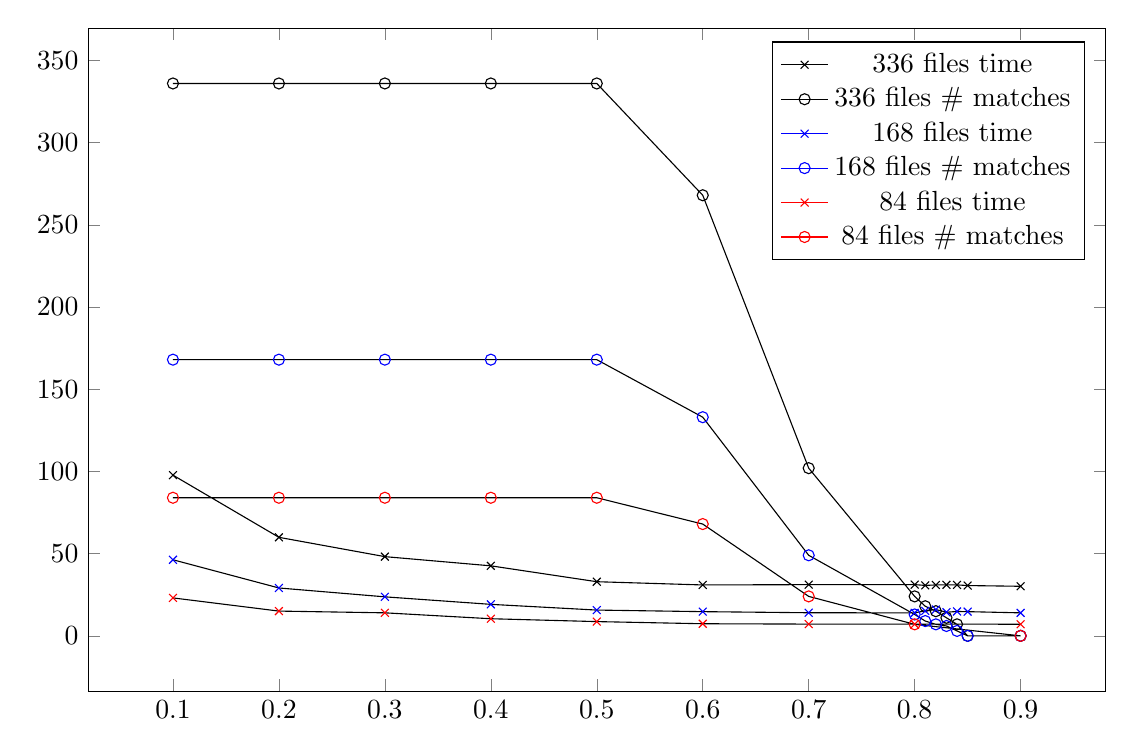
\begin{tikzpicture}
\begin{axis}[%
scatter/classes={%
    a={mark=x,draw=black},
    c={mark=o,draw=black},
    b={mark=x,draw=blue},
    d={mark=o,draw=blue},
    e={mark=x,draw=red},
    f={mark=o,draw=red}},width=14.5cm,height=10cm]
\addplot[scatter,%
    scatter src=explicit symbolic]%
table[meta=label] {
x y label
0.1 97.75 a
0.2 59.93 a
0.3 48.18 a
0.4 42.59 a
0.5 32.93 a
0.6 30.96 a
0.7 31.15 a
0.8 31.16 a
0.81 30.68 a
0.82 30.96 a
0.83 31.06 a
0.84 30.99 a
0.85 30.59 a
0.9 30.15 a

0.1 336 c
0.2 336 c
0.3 336 c
0.4 336 c
0.5 336 c
0.6 268 c
0.7 102 c
0.8 24 c
0.81 18 c
0.82 15 c
0.83 11 c
0.84 7 c
0.85 0 c
0.9 0 c

0.1 46.28 b
0.2 29.12 b
0.3 23.73 b
0.4 19.16 b
0.5 15.68 b
0.6 14.72 b
0.7 14.05 b
0.8 13.98 b
0.81 15.22 b
0.82 16 b
0.83 14.37 b
0.84 14.82 b
0.85 14.72 b
0.9 13.99 b

0.1 168 d
0.2 168 d
0.3 168 d
0.4 168 d
0.5 168 d
0.6 133 d
0.7 49 d
0.8 13 d
0.81 9 d
0.82 7 d
0.83 6 d
0.84 3 d
0.85 0 d
0.9 0 d

0.1 23.08 e
0.2 15.06 e
0.3 14.00 e
0.4 10.41 e
0.5 8.67 e
0.6 7.36 e
0.7 7.15 e
0.8 7.12 e
0.9 7.08 e

0.1 84 f
0.2 84 f
0.3 84 f
0.4 84 f
0.5 84 f
0.6 68 f
0.7 24 f
0.8 7 f
0.9 0 f
    };
\addlegendentry{336 files time}
\addlegendentry{336 files \# matches}
\addlegendentry{168 files time}
\addlegendentry{168 files \# matches}
\addlegendentry{84 files time}
\addlegendentry{84 files \# matches}
\end{axis}
\end{tikzpicture}
\caption{Number of Matches Found (number) and Speed of Matching (seconds) vs. Confidence Level For Varying Amounts of Training Images}
\end{figure}
\subsubsection{Distance Estimation}
\subsubsection{Environment Model Generation}
\subsubsection{User-Facing Application}

\section{Results}
\label{S:5}
\subsection{Algorithmic Analyses}
\subsubsection{Computer Stereo Vision}
\subsubsection{Structure-From-Motion Pipeline}
\subsubsection{Constellation}
Constellation's increased speed is due in part to its superior algorithmic efficiency. First consider its core object detection system, a neural network. The network is pre-trained, so in the analysis of its efficiency, the training steps, including the backpropagation algorithm used to fine tune its weights, will be ignored, as at run-time, they will not play any role in the time and number of calculations it takes to determine the nature of an object. Thus, the complexity of identifying an object is only the complexity of feeding the data from the image through the neural network and producing an output. Below is an abridged psuedocode version of the the feed-forward neural network algorithm:
\begin{program}
create\enspace an\enspace empty\enspace list\enspace of\enspace all\enspace layers'\enspace output
for\enspace each\enspace layer\enspace in\enspace the\enspace network:
\enspace\enspace	create\enspace an\enspace empty\enspace list\enspace of\enspace this\enspace layer's\enspace outputs
\enspace\enspace	calculate\enspace the\enspace biased\enspace input
\enspace\enspace	for\enspace each\enspace neuron\enspace in\enspace the\enspace layer:
\enspace\enspace\enspace\enspace		calculate\enspace output\enspace given\enspace biased\enspace input
\enspace\enspace\enspace\enspace		add\enspace ouput\enspace to\enspace list\enspace of\enspace this\enspace layer's\enspace outputs
\enspace\enspace	add\enspace this\enspace layer's\enspace output\enspace to\enspace list\enspace of\enspace all\enspace outputs
return\enspace all\enspace layers'\enspace outputs
\end{program}
The derivations and declarations of variables used to figure the complexity of the feed-forward algorithm are:
$$\text{\# layers}=\text{constant }c \enspace (\text{in our implementation }c=5)$$
$$\frac{\text{\# neurons}}{\text{layer}}=\sqrt{n}\text{ for $n$ elements in an input feature vector}$$
$$\frac{\text{\# calculations}}{\text{neuron}}=n+5$$
$$\text{\# times object detection called}=(w-\sqrt{n})(h-\sqrt{n})$$
$$\text{(for image width }w\text{, and image height }h;$$
$$\text{in our implementation }w=1080\text{, }h=720)$$
Thus, it can be determined that the complexity of determining the classification of a set of $n$ inputs is $O(5\sqrt{n}n+25\sqrt{n})$, and further, the complexity of classifying all objects in an image is $O(5\sqrt{n}n+25\sqrt{n})$. 

To perform similar tasks, a fairly naive implementation of a Structure-From-Motion pipeline would require $15n^3$ calculations, and a stereo vision system implementation would require $find\enspace this$ calculations, both far more than Constellation's mere $find\enspace this$ needed calculations.
\subsection{Implemented Executi{}on Time}
\subsection{Environment Accuracy}

\section{Conclusion}
\label{S:6}
\subsection{Advantages Over Similar Systems}
\subsection{Shortcomings and Future Improvements for Constellation}
- need to pre-train the network on objects before Constellation can put it in the environment accurately

- non-visual dot projection (infared or something else)

- increase time efficiency by concurrently carrying out object detection and dot detection operations (weight the pros and cons of distributed computations at that scale and their intensiveness on cpu, also weave in gpu acceleration)

- range, increase by stronger lasers and more training data for KNN model

%% The Appendices part is started with the command \appendix;
%% appendix sections are then done as normal sections
%% \appendix

%% \section{}
%% \label{}

%% References
%%
%% Following citation commands can be used in the body text:
%% Usage of \cite is as follows:
%%   \cite{key}          ==>>  [#]
%%   \cite[chap. 2]{key} ==>>  [#, chap. 2]
%%   \citet{key}         ==>>  Author [#]

%% References with bibTeX database:

%%\bibliographystyle{model1-num-names}
%%\bibliography{sample.bib}

%% Authors are advised to submit their bibtex database files. They are
%% requested to list a bibtex style file in the manuscript if they do
%% not want to use model1-num-names.bst.

%% References without bibTeX database:

% \begin{thebibliography}{00}

%% \bibitem must have the following form:
%%   \bibitem{key}...
%%

% \bibitem{}

% \end{thebibliography}


\end{document}

%%
%% End of file `elsarticle-template-1-num.tex'.